% Tipo de documento
\documentclass[16pt,spanish]{article}

% Codificación
\usepackage[utf8]{inputenc}
\usepackage[spanish,activeacute]{babel}

% Paquetes
\usepackage{graphicx}
\usepackage{float}
\usepackage[left=3cm,top=2.5cm,right=2.5cm,bottom=2.5cm]{geometry}

% Título, autor y fecha
\title{IberOgre y Sion Tower}
\author{David Saltares Márquez}


% Variables a usar para mantener un sistema consistente
\def \proyecto{\emph {IberOgre y Sion Tower} }
\def \juego{\emph {Sion Tower} }
\def \wiki{\emph{IberOgre} }


\begin{document}

% Título

\thispagestyle{empty}	

\begin{center}
    
    \makeatletter
    {\bf {\Huge \@title}}\\[1.5cm]
    {\bf {\Large Resumen para prensa}}\\[2cm]
    \begin{tabular}[t]{c} \@author \end{tabular}\\[2cm]
           
    \@date\\[12cm]

    
\includegraphics[scale=0.9]{img/by-nc-sa.png}
    
\end{center}

\cleardoublepage

\tableofcontents

\cleardoublepage

%\maketitle


%\begin{figure}[H]
%   \centering
%        
\includegraphics[width=2cm]{img/by-nc-sa.png} 
%    \label{img:licencia}
%\end{figure}

\paragraph{}

\section{Introducción}

\paragraph{IberOgre}
es una wiki en español sobre desarrollo de videojuegos en 3D
utilizando el motor de renderizado Ogre. Surge principalmente ante la
inexistencia de documentación al respecto en castellano. No solo está
dirigida a cubrir el uso del mencionado motor sino que también trata
los conceptos matemáticos y físicos mínimos para desarrollar juegos
tridimensionales.

\paragraph{}
\wiki se aloja en los servidores de la Oficina de Software Libre de la
Universidad de Cádiz (OSLUCA):

\begin{verbatim}
    http://osl2.uca.es/iberogre
\end{verbatim}


\begin{figure}[H]
    \centering
        
\includegraphics[width=7cm]{img/iberogre.png} 
    \caption{Logo del proyecto \wiki}
    \label{img:logo-iberogre}
\end{figure}

\paragraph{Sion Tower}
es un videojuego de estrategia y acción multiplataforma (GNU/Linux y Windows)
en 3D con elementos de fantasía cuyo objetivo principal es servir
de ejemplo final a \wiki. Controlamos
a un joven mago que debe defender la Torre Sagrada de una invasión mientras
sus compañeros están celebrando un rito. Cada nivel corresponde a un piso
de la torre y el objetivo consiste en evitar que los enemigos lleguen al
centro del mismo empleando hechizos y colocando trampas.

\paragraph{}
Está desarrollado en C++ utilizando bibliotecas libres como Ogre, OIS, SDL,
SDL mixer y pugixml. 

\begin{figure}[H]
    \centering
        
\includegraphics[width=9cm]{img/siontower.png} 
    \caption{Logo del proyecto \juego}
    \label{img:logo-siontower}
\end{figure}


\section{IberOgre}

\subsection{Motivaciones y objetivos}

\paragraph{}
El objetivo principal de \wiki es cubrir el vacío de \textbf{documentación en castellano}
sobre videojuegos en 3D. Así mismo, se pretende ofrecer especial soporte
al desarrollo con herramientas libres. Ningún texto será una traducción
de la wiki oficial, todos \textbf{los artículos serán originales}. La sección de
matemáticas busca que el lector no se vea obligado a recurrir a varias
fuentes distintas y disponga de todo lo necesario para comenzar en el
mismo lugar.

\paragraph{}
\wiki está dirigido a aquellos usuarios con un mínimo de experiencia en
creación de juegos bidimensionales que quieran dar el salto a las 3D. Podría
plantearse como una extensión de  \emph{Wikijuegos}\footnote{Wikijuegos: http://osl.uca.es/wikijuegos}, una wiki sobre
desarrollo de videojuegos en 2D utilizando libSDL alojada también en la OSLUCA.

\paragraph{}
El aprendizaje debía ser eminentemente práctico por lo que \wiki ofrecería
ejemplos de todos los temas tratados. Por supuesto, pretende emplear
buenas prácticas para el desarrollo multiplataforma (GNU/Linux y Windows
por el momento). No obstante, por encima de todo, el deseo es crear una
\textbf{comunidad} que aprenda a utilizar Ogre y colabore activamente en la creación de nuevo
contenido.

\begin{figure}[H]
    \centering
        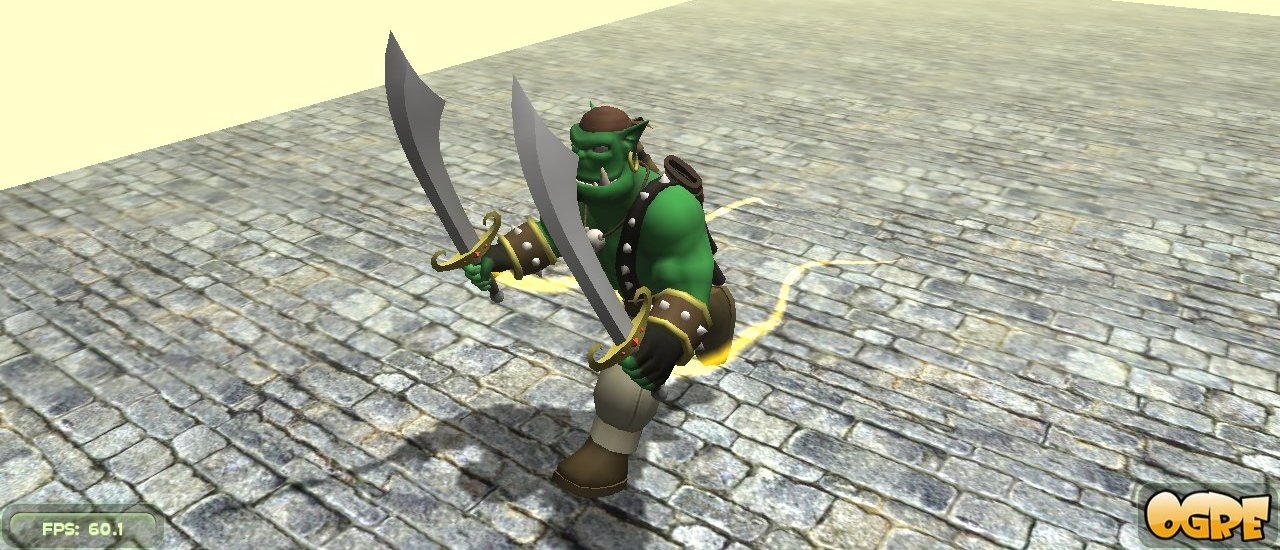
\includegraphics[width=10cm]{img/animaciones-iberogre.jpg} 
    \caption{Ejemplo de animaciones en IberOgre}
    \label{img:animaciones-iberogre}
\end{figure}

\subsection{Artículos}

\paragraph{}
Los artículos de \wiki están divididos en tres secciones principales bien
diferenciadas:

\begin{itemize}
    \item \textbf{Programación de videojuegos 3D}: artículos sobre matemáticas
    para el desarrollo de juegos tridimensionales. Centrado sobre todo en
    conceptos de álgebra y geometría del espacio, siempre ofreciendo aplicaciones
    prácticas.
    \item \textbf{Ogre 3D}: textos explicando cada uno de los aspectos más
    relevantes del motor de renderizado libre.
    \item \textbf{Otras tecnologías}: artículos sobre bibliotecas y herramientas
    que complementan a Ogre como manejo de dispositivos de entrada, audio,
    colisiones, etc.
\end{itemize}

\paragraph{}
Todos los artículos suelen compartir la misma estructura lógica. En primer
lugar se hace una introducción al lector sobre los temas a tratar y se
le indican los prerrequisitos, es decir, artículos que debería leer con
carácter previo antes del actual. En el bloque principal se desgrana
un subsistema de Ogre con pequeños ejemplos de código. Finalmente se concluye
con un ejemplo descargable de mayor complejidad que el lector debería
estudiar, comprender y, si es posible, modificar para experimentar.

\begin{figure}[H]
    \centering
        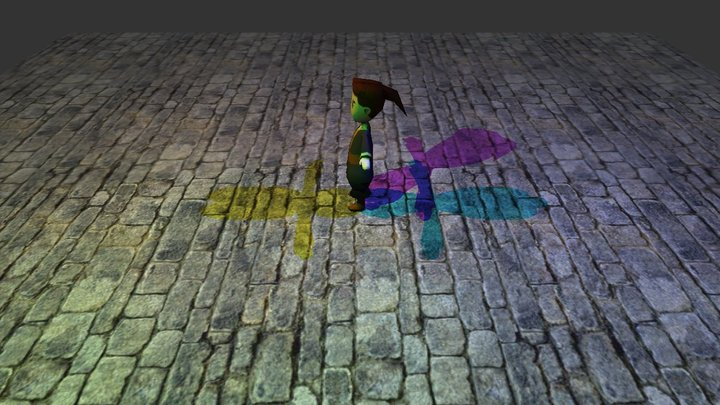
\includegraphics[width=8cm]{img/iluminacion-iberogre.jpg} 
    \caption{Ejemplo de iluminación en IberOgre}
    \label{img:iluminacion-iberogre}
\end{figure}

\subsection{Comunidad y colaboraciones}

\paragraph{}
El número de colaboraciones en \wiki está siendo bastante satisfactorio
y se espera que crezca con la difusión que proporciona el \emph{CUSL}.

\begin{itemize}
    \item \textbf{Artículo \emph{Conceptos generales}}: Alberto Cejas,
    participante del V CUSL con Fútbol es Así, ha redactado este texto
    en su totalidad.
    \item \textbf{Artículo \emph{Colisiones con OgreBullet}}: de nuevo,
    Alberto Cejas también ha compuesto este texto sobre detección de colisiones
    y simulaciones físicas.
    \item \textbf{Guía de Wikimedia}: Noelia Sales y Emilio José
    Rodríguez confecionaron una guía liberada bajo Creative Commons
    3.0 by-sa con los conocimientos básicos para la edición de artículos en
    instancias de Wikimedia.
    \item \textbf{Manual oficial}: Mario Velázquez Muñoz,
    alumno de la Universidad Carlos III de Madrid, aportó una traducción
    completa del manual de referencia oficial de Ogre. La traducción formaba
    parte de la documentación de su Proyecto Fin de Carrera y está disponible
    en la portada de \wiki bajo Creative Commons 3.0 by-nc-sa.
    \item \textbf{Ediciones}: \wiki cuenta con varios usuarios activos
    que han hecho correcciones y han aportado contenido adicional.
\end{itemize}

\section{Sion Tower}

\subsection{Motivaciones y objetivos}

\paragraph{}
La labor de \juego es ser una aplicación lo más realista posible de todos
los conocimientos expuestos en \wiki. Cada uno de los aspectos del desarrollo
está siendo completamente documentado para que los usuarios puedan ver
un \textbf{caso práctico de videojuego} con Ogre.

\paragraph{}
El deseo personal de crear videojuegos 3D se une a la inquietud de trabajar
en un \textbf{equipo multidisciplinar}: programación, audio, arte 3D, etc. En todo
momento se han buscado colaboradores para el apartado artístico.

\paragraph{}
El sistema que utiliza \juego es extensible y está orientado a la creación
de contenido adicional, como niveles diseñados con Blender. Sus componentes
son altamente reutilizables y lo deseable es que se liberen de forma
independiente para que cualquiera pueda integrarlos en su propio proyecto.
Entre estos componentes podrían citarse el sistema de audio 3D o el motor
de colisiones.

\begin{figure}[H]
    \centering
        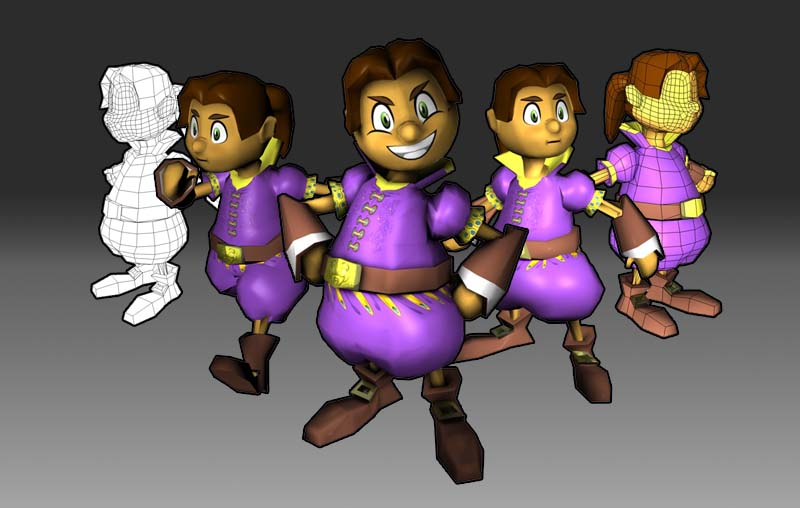
\includegraphics[width=10cm]{img/protagonista-siontower.jpg} 
    \caption{Protagonista de \juego}
    \label{img:protagonista-siontower}
\end{figure}


\subsection{Desarrollo}

\paragraph{}
El desarrollo de \juego comenzó con la elaboración de un \textbf{Documento
de Diseño} en el que se explicaban las mecánicas de juego, los personajes
y se listaba el arte necesario. Este documento fue de gran ayuda a la hora
de buscar colaboradores. Puede descargarse desde:

\begin{verbatim}
    http://forja.rediris.es/frs/download.php/2019/gdd.pdf
\end{verbatim}

\paragraph{}
Se ha desarrollado un \textbf{sistema de audio 3D} altamente
reutilizable y liberado de forma independiente. Cuenta con las siguientes
funcionalidades:

\begin{itemize}
    \item Reproducción de música en formato OGG y efectos en formato WAV.
    \item Integración completa con Ogre.
    \item Audio 3D: el volumen y el efecto estéreo dependen de la distancia
    y ángulo entre el emisor y el receptor.
\end{itemize}

\begin{figure}[H]
    \centering
        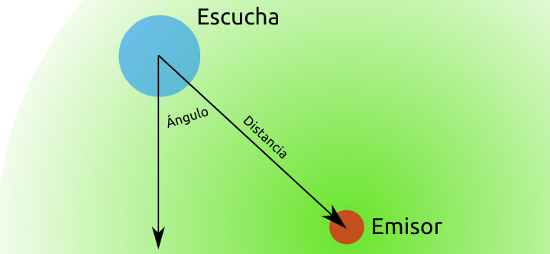
\includegraphics[width=8cm]{img/audio3d.png} 
    \caption{Sistema de audio 3D}
    \label{img:audio3d}
\end{figure}

\paragraph{}
\juego también cuenta con un sistema de \textbf{detección de colisiones} propio
que también ha sido liberado de forma independiente junto a su documentación.
Entre sus funcionalidades se encuentran:

\begin{itemize}
    \item Cuerpos colisionables compuestos de formas básicas: cajas, esferas...
    \item Detección automática de colisiones.
    \item Filtrado de colisiones: sólo se comprueban colisiones entre cuerpos
    del tipo deseado.
    \item Callbacks: podemos definir manejadores de eventos que se disparan
    ante la detección de un tipo concreto de colisión.
\end{itemize}

\begin{figure}[H]
    \centering
        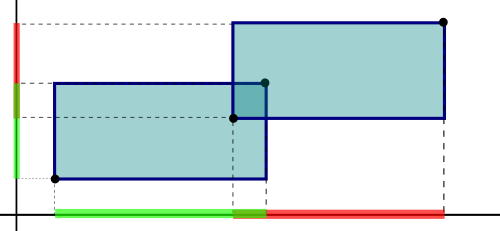
\includegraphics[width=8cm]{img/test-aabb-aabb.png} 
    \caption{Ejemplo de colisiones entre cajas sencillas}
    \label{img:colisiones}
\end{figure}

\paragraph{}
\juego está orientado a la creación de contenido por lo que se ha desarrollado
un sistema de \textbf{carga de niveles}. Cualquier persona sin conocimientos
de programación puede diseñar un nivel desde Blender y cargarlo dentro
del juego. Es posible definir los objetos que componen la escena, la música
que sonará, qué enemigos y cuándo aparecerán, etc.

\begin{figure}[H]
    \centering
        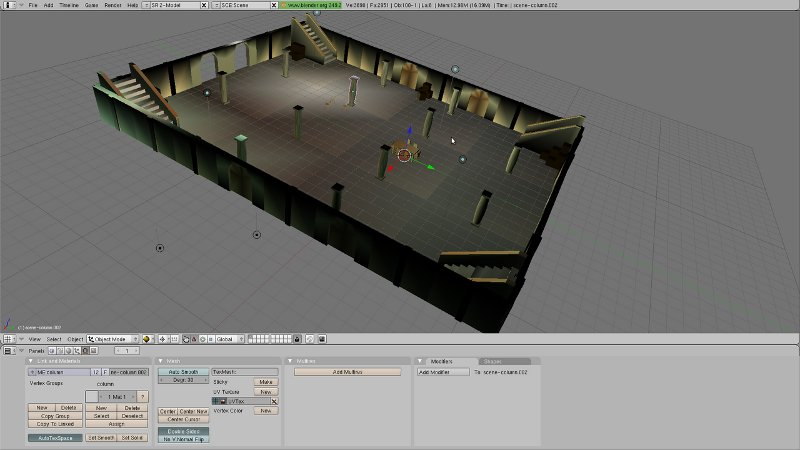
\includegraphics[width=10cm]{img/niveles-blender.jpg} 
    \caption{Creación de niveles desde Blender}
    \label{img:blender}
\end{figure}

\paragraph{}
Se ha publicado una \textbf{demo técnica de \juego} en la que el usuario
puede manejar a un prototipo de personaje por un escenario sencillo. Se
muestra en funcionamiento los sistemas de detección de colisiones, carga
de escenarios y audio. Desde su publicación, el proyecto ha evolucionado
pero aún puede descargarse desde:

\begin{verbatim}
http://forja.rediris.es/frs/download.php/2151/siontower-0.1-demo-src.tar.gz
http://forja.rediris.es/frs/download.php/2152/siontower-0.1-demo-win.zip
\end{verbatim}

\begin{figure}[H]
    \centering
        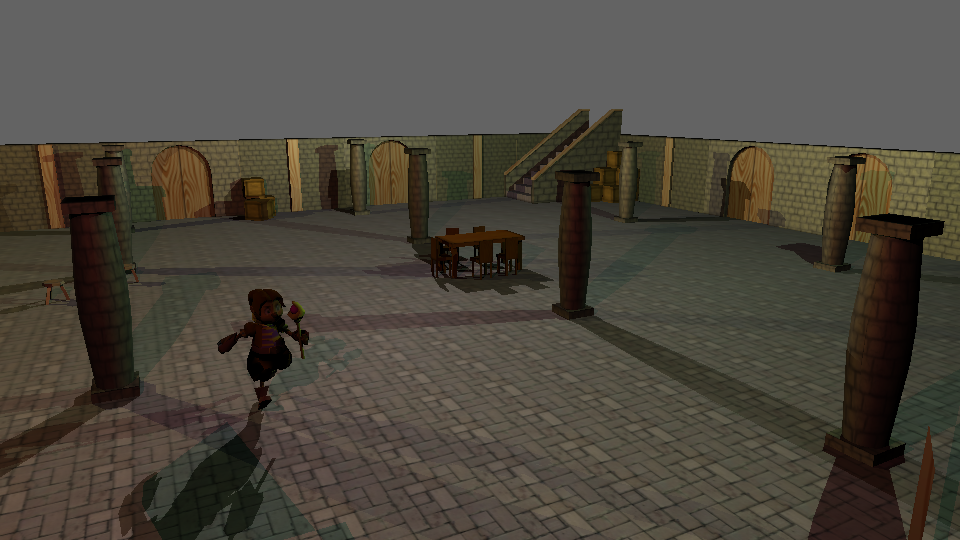
\includegraphics[width=10cm]{img/siontower-demo.png} 
    \caption{Demo técnica de \juego}
    \label{img:siontower-demo}
\end{figure}

\subsection{Colaboraciones}

\paragraph{}
Hasta la fecha, el proyecto \juego ha recibido varias colaboraciones, sobre
todo en el aspecto artístico. A continuación se listan los principales
contribuyentes:

\begin{itemize}
    \item \textbf{Arte 3D}: Antonio Jiménez, diseñador gráfico profesional 
    es el encargado del diseño, modelado, texturizado y animación de todos los personajes
    del juego.
    \item \textbf{Banda sonora}: el Estudio Evergreen, formado por Antonio Caro y Daniel
    Pellicer están componiendo una BSO completa para \juego.
    \item \textbf{Suavizado de caminos}: Javier Santacruz, estudiante de
    Ingeniería Informática, ha mejorado el suavizado de las rutas en el
    sistema de búsqueda de caminos de la IA.
\end{itemize}

\begin{figure}[H]
    \centering
        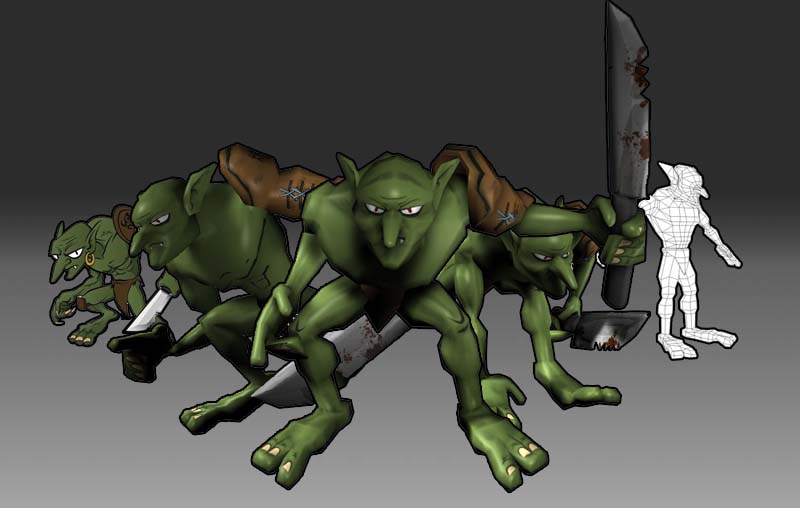
\includegraphics[width=10cm]{img/collage-goblin.jpg} 
    \caption{Enemigo Goblin de \juego diseñado por AJR}
    \label{img:collage-goblin}
\end{figure}


\section{Difusión}

\paragraph{}
El proyecto ha sido mencionado en un buen número de medios relacionados
con el desarrollo de videojuegos:

\begin{itemize}
    \item \textbf{Comunidades de desarrollo}: varias comunidades de desarollo
    de videojuegos en español han publicado artículos hablando de \proyecto.
    \begin{verbatim}
    http://www.creagames.es/iberogre-un-proyecto-espanol-de-ogre-engine
    http://razonartificial.com/2011/03/iberogre-documentacion-de-ogre-en-espanol
    http://programandoideas.com/2011/01/iberogre-tutoriales-de-ogre3d-en-espanol
    \end{verbatim}
    \item \textbf{Web oficial de Ogre}: \wiki apareció en la portada de
    la web oficial de Ogre dentro de la cuarta sección de noticias.
    \begin{verbatim}
    http://www.ogre3d.org/2011/03/01/ogre-news-4
    \end{verbatim}
    \item \textbf{Twitter}: 79 seguidores de los que se han recibido muchas
    sugerencias y opiniones. Steve Streeting, fundador de Ogre, recomendó
    \wiki a través de este medio.
    \item \textbf{Blog}: más de 70 artículos con 58.000 visitas en el
    periodo del concurso.
    \item \textbf{Medios tradicionales}: tras el anuncio de los finalistas
    del V CUSL, \proyecto ha sido mencionado en periódicos locales como Viva Cádiz
    y Bahía de Cádiz.
\end{itemize}

\section{Enlaces}

\paragraph{}
Se adjunta la lista de enlaces en los que encontrar información adicional
del proyecto.

\begin{figure}[H]
    \centering
        
\includegraphics[width=9cm]{img/enlaces.png} 
    \caption{Medios con información sobre \proyecto}
    \label{img:enlaces}
\end{figure}

\begin{itemize}
    \item Blog: noticias, anuncios, experiencias, anécdotas y documentación.
    \begin{verbatim}http://siondream.com/blog/category/proyectos/pfc\end{verbatim}
    \item Forja: descargas de versiones, repositorio Subversion, noticias, y gestión de tareas.
    \begin{verbatim}https://forja.rediris.es/projects/cusl5-iberogre\end{verbatim}
    \item Web de la forja: información básica y enlaces a todos estos medios
    \begin{verbatim}http://cusl5-iberogre.forja.rediris.es\end{verbatim}
    \item Twitter: noticias, detalles del desarrollo y contacto cercano
    con los seguidores del proyecto.
    \begin{verbatim}http://twitter.com/iberogre\end{verbatim}
    \item Canal de Youtube: vídeos mostrando el desarrollo de \juego.
    \begin{verbatim}http://youtube.com/user/davidsaltares\end{verbatim}
\end{itemize}

\end{document}
